\subsection{Real Estate Investments}

\subsubsection{Overview of Real Estate Investments}

\begin{remark} \hlt{Types of Real Estate}
\begin{enumerate}[label=\roman*.]
\setlength{\itemsep}{0pt}
\item Residential: single-family homes, apartments, condominiums, manufactured housing
\item Non-Residential Property: office, shopping centres, factories, warehouses, agriculture, specialty real estate
\end{enumerate}
\end{remark}

\begin{figure}[H]
\centering
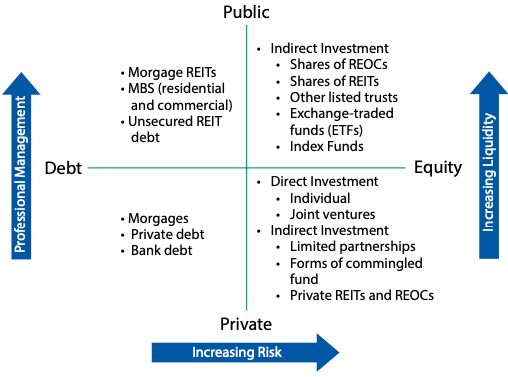
\includegraphics[scale=0.4]{/alts/reinvestments}
\caption{Forms of Real Estate Investments}
\end{figure}

\begin{remark} \hlt{Private vs Public Real Estate}
\begin{enumerate}[label=\roman*.]
\setlength{\itemsep}{0pt}
\item Public Real Estate: ownership on securities that serve as claims on underlying.
\begin{enumerate}[label=\arabic*.]
\setlength{\itemsep}{0pt}
\item Real Estate Investment Trust (REIT): restricted to primarily owning and operating rental properties, or purchasing mortgages. Required to distribute all earnings to avoid paying corporate income taxes.
\item Real Estate Operating Company (REOC): taxable corporations that operate and manage commercial real estate with few corporate-structure restrictions. Own and often develop real estate.
\item Mortgage-Backed Securities (MBS): classified as public investments when there are active secondary trading markets. Restrictions exist as to purchase eligibility and minimum trade sizes. Trust certificate owners (bondholders) typically own right to receive cash flow from underlying pool of mortgages, which are secured by real property.
\end{enumerate}
\item Private Real Estate: direct investment by purchasing property or lending money to purchaser. Can be solely owned or owned through partnerships, where GP provides property management services.
\end{enumerate}
\end{remark}

\begin{remark} \hlt{Capital Position}
\begin{enumerate}[label=\roman*.]
\setlength{\itemsep}{0pt}
\item Equity investor has ownership interest in real estate or securities of an entity that owns real estate. Controls decisions such as borrowing money, property management, exit strategy.
\item Debt investor owns mortgage or mortgage securities, usually secured by the underlying. Lender has superior claim over equity investor during default.
\end{enumerate}
As lender has to be repaid first, value of equity interest is value of property less outstanding debt.
\end{remark}

\begin{remark} \hlt{Characteristics of Real Estate Investment}
\begin{enumerate}[label=\roman*.]
\setlength{\itemsep}{0pt}
\item Heterogeneity: no two RE are the same due to size, age, construction materials, tenants, lease terms
\item High Unit Value: RE is indivisible, unit value is higher, hence difficult to construct diversified portfolio
\item Active Management: private Re investment require active property management, which involves maintenance, negotiating leases, collection of rents
\item High Transaction Costs: involves appraisers, lawyers, brokers, construction personnel
\item Depreciation: less desirable due to location, design, or obsolescence. Deductibility of depreciation for tax purposes is attractive feature for investors in most jurisdictions
\item Illiquidity: takes time to market and complete sale of property
\item Need for Debt Capital: due to high costs of acquisition. RE values are lower when interest rates are high and debt capital is scarce
\item Price Determination: due to heterogeneity and low transaction volume, appraisals are required, which is based on similar but not identical properties. Market is less efficient. Limited participants, importance  of local knowledge, makes it harder to know market value of a property
\end{enumerate}
\end{remark}

\begin{remark} \hlt{Demand and Supply Risk Factors of Commercial Real Estate}
\begin{enumerate}[label=\roman*.]
\setlength{\itemsep}{0pt}
\item Business Conditions: GDP, employment, household income, interest rates, inflation affect rental
\item Demographics: shifts in size and age distribution affect type of property in demand. Changes in socioeconomic groups and rate of new household formation all affect demand.
\item Excess Supply: market conditions can change significantly while approvals are obtained, while property is completed, and when property is fully leased.\\
During lead time, if market conditions weaken, lower demand affects rents and vacant rates, resulting in lower returns. Commercial property demand coincide with business cycle.
\end{enumerate}
\end{remark}

\begin{remark} \hlt{Valuation Risk Factors of Commercial Real Estate}
\begin{enumerate}[label=\roman*.]
\setlength{\itemsep}{0pt}
\item Cost and Availability of Capital: RE must compete with other investments for capital. Demand for RE is reduced when debt capital is scarce, interest rates are high.
\item Availability of Information: lack of info to conduct property analysis adds to risk of investment. Availability of data depends on country. More information is available as RE investments become more global.
\item Lack of Liquidity: due to size and complexity of transactions, due diligence takes time and is costly. Quick sale will require significant discount.
\item Interest Rates: RE values may initially decline when interest rates rise, but may increase over time through the latter part of the RE cycle.
\end{enumerate}
\end{remark}

\begin{remark} \hlt{Operational Risk Factors of Commercial Real Estate}
\begin{enumerate}[label=\roman*.]
\setlength{\itemsep}{0pt}
\item Management Expertise: property managers and asset managers must take important operational decisions, such as lease negotiation, property maintenance, marketing, property renovation.
\item Lease Provisions: pre-determined contractual rent step-ups can move in line with unexpected inflation if tied to consumer price or other inflation-linked index. Expense caps will limit how much of annual increase of operating expenses is passed to tenant. Short-term leases allow periodic rent reviews in response to changing market conditions.
\item Leverage: use of leverage to finance real estate affect returns but not value of underlying RE. Loan-to-value (LTV) ratio (ratio of borrowed funds to total purchase price) measure leverage, with higher LTV resulting in higher leverage hence higher risk. With leverage, small decrease in net operating income (NOI) negatively magnifies amount of CF available to equity investors after debt service.
\item ESG Considerations: RE values may be affected by environmental conditions. Social and governance-related issues may impact development and management of RE.
\item Obsolescence: Changes in tenant preferences, regulations, technology affect space demand. May not be economically viable to upgrade, reconfigure, or repurpose old buildings to comply with energy efficiency and other modernisation requirements or changing business and consumer preferences.
\item Market Disruptions: new innovations such as remote working, online shopping, same-day delivery and other disruptions affect the demand for various kinds of real estate.
\item Other Risk Factors: unobserved physical defects in property, natural disasters, pandemics, terrorism, climate change may be unidentified and difficult-to-forecast at time of purchase.
\end{enumerate}
\end{remark}

\begin{remark} \hlt{Reasons to Invest in Real Estate}
\begin{enumerate}[label=\roman*.]
\setlength{\itemsep}{0pt}
\item Current Income: earn income from letting, leasing, or renting, after paying operating expenses, financing costs, and taxes. Usually largest component of investor return.
\item Capital Appreciation: property values may increase over time, which forms part of total return
\item Inflation Hedge: both rents and property values expected to rise in inflationary environment
\item Diversification: not typically highly correlated with performance of other asset classes, hence may reduce risk relative to expected return. Publicly traded RE behaves more like stock in the short-run.
\item Tax Benefits: private RE investments may receive favourable tax treatment. In US, RE can be depreciated for tax purposes faster than actual life. In some countries, REITs do not may income taxes if income is distributed ($> 90\%$) to shareholders.
\end{enumerate}
\end{remark}

\begin{remark} \hlt{Role of Real Estate in Portfolio}\\
RE has both bond and stock characteristics. Leases call for periodic rental payments, similar to coupon payments of a bond. As lease expires, there is uncertainty on renewal and future rental rates. Availability of competing space, tenant profitability, state of overall economy affect this uncertainty just as these factors affect stock prices. Hence RE risk-return profile is between risk-return profile of stocks and bonds.
\end{remark}

\begin{remark} \hlt{Core Investing Style}\\
A conservative strategy that limits investments to high quality and low leverage ($< 30\%$ LTV), and avoids speculative risks in favour of steady returns.
\end{remark}

\begin{remark} \hlt{Economic Value Determinants of Real Estate Investments}\\
National GDP growth is largest driver of economic value for all RE types, as this means more jobs, greater need for office space, more disposal income, more growth in shopping centres, greater demand for hotel rooms etc.
\end{remark}

\begin{flushleft}
Economic Value Determinants
\begin{tabularx}{\textwidth}{p{10em}|p{12em}|p{6em}|p{2.5em}|p{2.5em}|p{2.5em}|p{4.5em}}
\hline
\rowcolor{gray!30}
Factor Type & Factor & Multi-Family & Retail & Hotel & Office & Industrial \\
\hline
Macro & GDP Growth & $\checkmark$ & $\checkmark$ & $\checkmark$ & $\checkmark$ & $\checkmark$ \\
& Population Growth & $\checkmark$ & $\checkmark$ & $\checkmark$ & $\checkmark$ & $\checkmark$ \\
& Job Creation & $\checkmark$ & $\checkmark$ & $\checkmark$ & $\checkmark$ & $\checkmark$ \\
& Wage Growth & $\checkmark$ & $\checkmark$ & $\checkmark$ & $\checkmark$ & $\checkmark$ \\
& Regulatory & $\checkmark$ & $\checkmark$ & $\checkmark$ & $\checkmark$ & $\checkmark$ \\
& Taxes & $\checkmark$ & $\checkmark$ & $\checkmark$ & $\checkmark$ & $\checkmark$ \\
\hline
Individual & Household Formations & $\checkmark$ & $\checkmark$ & & & \\
& Personal Income & $\checkmark$ & $\checkmark$ & $\checkmark$ & & \\
& Consumer Confidence & $\checkmark$ & $\checkmark$ & $\checkmark$ & & \\
& Consumer Credit & $\checkmark$ & $\checkmark$ & $\checkmark$ & & \\
\hline
Business Environment & Retail Sales Growth & & $\checkmark$ & & & $\checkmark$ \\
& Consumer Spending & & $\checkmark$ & $\checkmark$ & & $\checkmark$ \\
& Business Formations & $\checkmark$ & & $\checkmark$ & $\checkmark$ & $\checkmark$ \\
& Business Investment & & & $\checkmark$ & $\checkmark$ & $\checkmark$ \\
& Business Confidence & & $\checkmark$ & $\checkmark$ & $\checkmark$ \\
\hline
Industrial & Industrial Production & & & & & $\checkmark$ \\
& Trade, Transport, Logistics & & & & & $\checkmark$ \\
& Changing Supply Routes & & & & & $\checkmark$ \\
\hline
\end{tabularx}
\end{flushleft}

\begin{remark} \hlt{Types of Leases}
\begin{enumerate}[label=\roman*.]
\setlength{\itemsep}{0pt}
\item Net Lease: tenant responsible for paying operating expenses.
\item Gross Lease: owner to pay operating expenses.
\item Triple-Net Lease (NNN): tenants to pay for share of common area maintenance (CAM) and repair expenses, property taxes, building insurance costs; also responsible for own furnishings, equipment, systems etc. against fire, water damage, and other perils.
\item Sales-Leaseback: long-term single-tenant lease requiring tenant to pay all expenses directly, in addition to base rent. Company sells building it owns and occupies to a RE investor and the company then signs long-term least with buyer to continue to occupy the building.
\end{enumerate}
\end{remark}

\begin{remark} \hlt{Commercial Property Classifications}
\begin{enumerate}[label=\roman*.]
\setlength{\itemsep}{0pt}
\item Residual Properties: multi-family and single-family properties that are not owner occupied, purchased with the intent to rent out to produce income.\\
Multi-family properties differentiated by location (urban, suburban), structure height (high-rise, mid-rise, low-rise, garden apartments, townhouses), amenities (pool, balcony, exercise facilities, concierge services).\\
Demand depends on population growth. Age demographic vary by country, type of property, locale. Cost of buying versus cost of renting, measured by ratio of home prices to rents, also affect demand.
\item Office: multi-tenant, or single-tenant. Built with needs of specific tenants in mind.\\
Demand heavily dependent on job growth, especially in industries that are heavy users of office space. Average length of office leases varies globally.
\item Industrial and Warehouse: wholesale and retail distribution centres, combination warehouse/showroom and office buildings, light or heavy manufacturing facilities and associated warehouse space.\\
Demand heavily dependent on overall economy. Import and export activities also affect demand.\\
Net leases are common.
\item Retail: vary significantly in size. Large regional shopping centres, malls with large department stores, big-box retailers, neighbourhood shopping centres, standalone properties.\\
Demand heavily dependent on consumer spending, which in turn depends on overall economy, job growth, population growth, savings rates.\\
Retail lease terms vary by quality of property, size and importance of tenant.\\
Retail tenant often required to pay additional rent when sales reach certain level (percentage lease or rent). Lease will specify minimum amount of rent to be paid without regard to sales. 
\item Hospitality: varies by size and available amenities. Motels, smaller hotels, resort hotels etc.
\item Other Specialty Types: hospitals, bioscience laboratories, self-storage, student housing, cell towers, data centres, parking facilities, marinas, sport complexes etc.
\end{enumerate}
Low-risk commercial property types include office, industrial/warehouse, retail, multi-family. Hospitality properties are riskier as leases are not used, and performance is highly correlated with business cycle.
\end{remark}

\begin{remark} \hlt{Property Due Diligence: Market Review}
\begin{enumerate}[label=\roman*.]
\setlength{\itemsep}{0pt}
\item Understand market trends, including local market population, job and income growth
\item Understand expected additions to supply and space absorption rates (how much net space is leased yearly)
\item Understand tenant preferences, building amenities, market rents, and expense trends.
\end{enumerate}
\end{remark}

\begin{remark} \hlt{Property Due Diligence: Lease and Rent Review}
\begin{enumerate}[label=\roman*.]
\setlength{\itemsep}{0pt}
\item Compare the tenant rents with market rent forecasts and lease length to determine how much rents will change when leases expire.
\item Review lease expiration timeline for all tenants. $~20\%$ of leases expire in any given year, or there may be some years with larger lease expirations.
\item Analyse the history of rental payments, late payments, and any defaults for the major tenants.
\end{enumerate}
\end{remark}

\begin{remark} \hlt{Property Due Diligence: Review Costs of Re-Leasing}\\
Review costs and incentives provided to both renewing and new tenants.
\begin{enumerate}[label=\roman*.]
\setlength{\itemsep}{0pt}
\item Costs: typically include commissions paid to real estate brokers and downtime between leases.
\item Incentives: typically include a period of free rent and allowances for tenant improvements to their space.
\end{enumerate}
These costs are typically not included in annual operating income. Instead, these expenses are capitalised and amortised over the length of the lease.
\end{remark}

\begin{remark} \hlt{Property Due Diligence: Review Documentation}
\begin{enumerate}[label=\roman*.]
\setlength{\itemsep}{0pt}
\item Review copies of bills for operating expenses, i.e., utility bills and real estate taxes.
\item Review multiple years of audited fin statements. CFS provide details on Opex and revenue trends.
\item Look for evidence of overstated income (Capex underspending) or occupancy (tenant incentives).
\end{enumerate}
\end{remark}

\begin{remark} \hlt{Property Due Diligence: Property Inspections and Service Agreements}
\begin{enumerate}[label=\roman*.]
\setlength{\itemsep}{0pt}
\item Conduct environmental inspection to check for issues, i.e., contaminant material.
\item Conduct physical and engineering inspection for structural issues. Check condition of systems, structures, and foundation and  adequacy of utilities.
\item Review service and maintenance agreements to determine whether recurring problems exist.
\item Conduct property survey to determine if the planned physical improvements are in the boundary lines of the site and to find out if any easements would affect the value.
\end{enumerate}
\end{remark}

\begin{remark} \hlt{Property Due Diligence: Legal Documentation and Tax Compliance}
\begin{enumerate}[label=\roman*.]
\setlength{\itemsep}{0pt}
\item Conduct title search by reviewing the ownership history. Make sure there are no issues related to the property title and that the property is not subject to any previously unidentified liens.
\item Verify that the property is compliant with zoning laws, environmental regulations, parking ratios etc.
\item Verify that property taxes, insurance, special assessments etc. have been paid.
\end{enumerate}
\end{remark}

\begin{method} \hlt{Appraisal-Based Indexes}\\
Index combine valuation from individual properties to provide measure of market movements.\\
In US, members of NCREIF (National Council of Real Estate Investment Fiduciaries) contribute appraised values, net operating income (NOI), capital expenditures and other information on a quarterly basis. The return for all properties is then calculated as
\begin{equation}
\text{Return} = \frac{\text{NOI} - Capex + (\text{Market Value}_{\text{End}} - \text{Market Value}_{\text{Beginning}})}{\text{Market Value}_{\text{Beginning}}} \nonumber
\end{equation}
The return is a holding-period return. The index is then value weighted based on returns of separate properties.
\end{method}

\begin{remark} \hlt{Characteristics of Appraisal-Based Indexes}\\
The index has a current yield component (NOI divided by beginning market value).\\
Remaining components of equation produce the capital return.\\
Note that the income component of return does not represent REIT distributions, unlike other asset classes.\\
The index lags actual transactions as transactions occur before appraisals are performed. The lag can be adjusted by un-smoothing the index or by using a transaction-based index.\\
Global RE index is a cap-weighted index that is published quarterly, and includes local currency return. Index combines data from US, Europe, and Asia.
\end{remark}

\begin{method} \hlt{Transaction-Based Indices}
\begin{enumerate}[label=\roman*.]
\setlength{\itemsep}{0pt}
\item Repeat-Sales Index: relies on repeat sales of same property. Change in market conditions can be measured once a property is sold more than once.\\
Regression may then be used to allocate change in value to each quarter.
\item Hedonic Index: requires only single sale data. Regression model controls for differences in property characteristics such as size, age, quality of construction, and location. Require a lot of data, most reliable at national level; may be reliable at regional level if sufficient transactions are available.
\end{enumerate}
\end{method}

\subsubsection{Publicly Traded Real Estate Investments}

\begin{remark} \hlt{Equity Real Estate Instruments}\\
Equity securities represent ownership stakes in properties.
\begin{enumerate}[label=\roman*.]
\setlength{\itemsep}{0pt}
\item Equity REITs: tax-advantaged companies (trusts) exempt from corporate income tax. Actively managed, own income-producing real estate, seek to profit by generating cash flows, improving existing properties, purchasing additional properties. Usually specialise in a particular property, diversifying holdings by geography and other factors. To be tax advantaged, required to distribute $> 90\%$ of taxable income.
\item Real Estate Operating Companies (REOCs): not tax advantaged; ordinary corporations that own RE. Business will form REOC if ineligible to form REIT, as the company may intend to develop and sell RE rather than generating cash from rental payments, offer non-qualifying services such as brokerage or third-party property management, or located in a country that does not allow tax-advantaged REITs.
\end{enumerate}
\end{remark}

\begin{remark} \hlt{Debt Real Estate Instruments}
\begin{enumerate}[label=\roman*.]
\setlength{\itemsep}{0pt}
\item Residential or Commercial Mortgage-Backed Securities (RMBS, CMBS): publicly traded asset-backed securitised debt obligations that receive CF from an underlying pool of mortgage loans. Represents a far larger aggregate market value than publicly traded RE equity.
\item Mortgage REITs: invest primarily in mortgages, mortgage securities, loans secured by RE.
\end{enumerate}
\end{remark}

\begin{remark} \hlt{REIT Structures}\\
To quality as a REIT, the requirements are as follows:
\begin{enumerate}[label=\roman*.]
\setlength{\itemsep}{0pt}
\item distribute $90\%$ to $100\%$ of otherwise taxable earnings
\item invest at least $75\%$ in RE
\item derive at least $75\%$ of income from RE rental income or interest on mortgages
\end{enumerate}
Require minimum number of shareholders, maximum share ownership by single shareholder, minimum number of properties, maximum asset concentration, maximum level of non-rental income, maximum amount of development, limits on leverage and types of loans.\\
In US, REIT must have at least $100$ shareholders, no fewer than five shareholders can own more than $50\%$ of shares ($5/50$ rule). Most REITs are self-managed and self-advised, which hav fewer conflicts than externally-managed or externally-advised REITs
\end{remark}

\begin{remark} \hlt{Advantages of REITs}
\begin{enumerate}[label=\roman*.]
\setlength{\itemsep}{0pt}
\item Liquidity: greater liquidity than that of physical real estate, as REIT trade on major exchanges
\item Transparency: readily available share price and transaction histories
\item Diversification: by property type, geography, underlying tenant credit
\item High=Quality Portfolios: companies own high-quality assets in leading markets
\item Active Portfolio Management: strong executive management overseeing dedicated property management teams with economies of scale
\item Potentially Stable Income: well-occupied properties with long-term leases generate predictable income
\item Tax Efficiency: avoid corporate income taxation, leaving investor to only pay taxes on dividends received
\end{enumerate}
\end{remark}

\begin{remark} \hlt{Disadvantages of REITs}
\begin{enumerate}[label=\roman*.]
\setlength{\itemsep}{0pt}
\item Lack of Retained Earnings: must access capital markets to fund growth. The faster the expansion, the more often the company must raise new capital.
\item Regulatory Costs: have cost burden of maintaining a corporate structure of publicly traded company and complying with regulatory filings.
\item Reduced Portfolio Diversification Benefits: REIT shares pricing are partially determined by stock market movements and liquidity rather than only by underlying value, unlike private RE
\item Limit in Types of Assets Owned: constrained in type of assets owned.\\
REITs form taxable REIT subsidiaries (TRS) which pay income taxes on earnings from non-REIT-qualifying activities such as merchant development or third-party property management 
\end{enumerate}
\end{remark}

\subsubsection{Net Asset Value Approach}

\begin{definition} \hlt{Net Asset Value Per Share (NAVPS) Approach}\\
Market-based approach, measures per-share amount by which assets exceed liabilities.\\
Considered most appropriate measure of fundamental value of REITs. If market price of REIT varies from NAVPS, premium/discount reflect investor's view of management capabilities, leverage and governance.\\
REITs with high leverage and trading at discount to NAVPS may find it difficult to refinance maturing debt.\\
Superior to Book Value per Share (NVPS) as it relies on depreciated historical cost of REIT asset.
\end{definition}

\begin{remark} \hlt{Valuation of Investment Properties: IFRS}
\begin{enumerate}[label=\roman*.]
\setlength{\itemsep}{0pt}
\item Cost Model: identical to cost model used for PP\&E
\item Fair Value Model: all changes in fair value affect net income. Requires reliability in determining property fair value on continuation basis. Once chosen for reporting, must continue usage of model until disposal of property or change in property use such that it is no longer investment property.
\end{enumerate}
Investment property is a separate line item on the balance sheet. Companies to disclose choice of model.\\
If fair value model is chosen, to make additional disclosures on how fair value is determined and must provide reconciliation between beginning and ending carrying amounts.\\
If cost model is used, depreciation method and useful life estimates must be disclosed. Must also disclose fair value of the investment property.
\end{remark}

\begin{remark} \hlt{Valuation of Investment Properties: GAAP}\\
Historical cost accounting model used, which values asset at original purchase price plus capital investment less historical depreciation. Model does not accurately represent economic values of assets and liabilities if there is significant operating income and asset price changes, or long-term inflation.\\
Method understates carrying values on long-held property assets often appreciating due to general price inflation or other property-specific reasons, and overstates depreciation when companies use accelerated depreciation.
\end{remark}

\begin{method} \hlt{Computing NAVPS with Net Operating Income (NOI)}\\
If reliable appraisal is unavailable, value of operating real estate holdings may be estimated by capitalising the REIT's cash net operating income (NOI).
First, calculate the market-required rate of return (Cap Rate), based on prices of comparable recent transactions that have taken place in the market.
\begin{align}
\text{Cap Rate} &= \frac{\text{NOI}_{\text{Comps}}}{\text{Transaction Price}_{\text{Comps}}} \nonumber \\
\text{NOI} = \text{Gross rental revenue} &- \text{Estimated vacancy and collection losses} - \text{Opex} \nonumber
\end{align}
NOI is calculated before subtracting financing costs, depreciation, general and admin expenses, income taxes.\\
To compute Cash NOI, subtract non-cash rent.
\begin{equation}
\text{Non-Cash Rent} = \text{Average rent over term of lease contract} - \text{Actual cash rent received} \nonumber
\end{equation}
To forecast NOI for next year, two adjustments are made to current period NOI:
\begin{enumerate}[label=\roman*.]
\setlength{\itemsep}{0pt}
\item impact of acquisitions for the current year, which are not fully reflected in current period NOI
\item growth rate
\end{enumerate}
\end{method}

\begin{flushleft}
Computing NAVPS from NOI
\begin{tabularx}{\textwidth}{X|p{25em}}
\hline
\rowcolor{gray!30}
Line Item & Comments \\
\hline
Last $12$ Month NOI & \\
$-$ Non-Cash Rents & Actual contractual rent $-$ cash rent paid \\
$+$ Full-year adjustment for acquisition & Full-year rent for properties acquired during the year \\
$=$ Pro-Forma cash NOI for last 12 month & \\
\hline
$+$ Next $12$-month growth in cash NOI & Estimated growth in cash NOI over next year \\
$=$ Estimated next 12-month cash NOI & \\
\hline
$\div$ Assumed cap rate & Based on recent transaction for comparables \\
$=$ Estimated value of operating real estate & \\
\hline
$+$ Cash and equivalents & \\
$+$ Land held for future development & \\
$+$ Accounts receivable & \\
$+$ Prepaid and Other Assets & Does not include intangible assets \\
$=$ Estimated gross asset value & \\
\hline
$-$ Total debt & \\
$-$ Other liabilities & \\
$=$ Net Asset Value & \\
\hline
$\div$ Shares outstanding & \\
$=$ Net Asset Value Per Share (NAVPS) & \\
\hline
\end{tabularx}
\end{flushleft}

\begin{remark} \hlt{Considerations in NAV-Based Approach to Valuing REITs}\\
Common methods used to calculate NAV are:
\begin{enumerate}[label=\roman*.]
\setlength{\itemsep}{0pt}
\item using cap rate approach to valuing NOI to property or portfolio of properties
\item applying value per square foot or unit to property or portfolio of properties
\item using appraised values disclosed in company's financial statements
\end{enumerate}
The appraised value may be adjusted if the underlying assumptions are not reliable. Cap rate and values per unit are derived from market transactions. Sophisticated direct purchasers will use detailed forecasting of cash flows expected to achieve from owning and operating a specific property to arrive at the NAV value.\\
Price-to-NAV ratio will vary by market, sector, outlook, perceived quality of management and governance.\\
Appraisal-based NAV approach lags changes in market conditions.\\
NAV implicitly treats a company as an individual asset or static pool of assets, which is not consistent with going-concern assumption. To consider how much value a management can add or subtract from current NAV.
\end{remark}

\begin{remark} \hlt{Relative Valuation using NAVPS}\\
Relative valuation with NAVPS is comparing NAVPS to market price of a REIT/REOC share. If market is trading at premium to NAVPS, select investments with lowest premium.
\end{remark}

\subsubsection{Price Multiple Approach}

\begin{definition} \hlt{Funds from Operations (FFO)}\\
FFO attempts to approximate continuing operating performance.\\
\begin{tabularx}{\textwidth}{p{25em}|X}
\hline
\rowcolor{gray!30}
Line Item & Comments \\
\hline
Accounting Net Income & \\
$+$ Depreciation, amortisation, impairments, write-downs & Accounting dep often $>$ economic dep \\
$-$ Gains from sales of property & Not considered part of continuing income \\
$+$ Loss from sales of property & Not considered part of continuing income \\
\hline
$=$ Funds from Operations (FFO) & \\
\hline
\end{tabularx}
Like cash flow form operations, FFO is not a measure of cash flow.
\end{definition}

\begin{definition} \hlt{Adjusted Funds from Operations (AFFO)}\\
Also known as funds available for distribution (FAD) or cash available for distribution (CAD). More accurate measure of current economic income.\\
\begin{tabularx}{\textwidth}{p{25em}|X}
\hline
\rowcolor{gray!30}
Line Item & Comments \\
\hline
Funds from Operations (FFO) & \\
$-$ Non-cash (straight-line) rent adjustment & $=$ average contractual rent $-$ rent actually paid \\
$-$ Recurring capex & Maintenance, leasing commissions \\
\hline
$=$ Adjusted Funds from Operations (AFFO) & \\
\hline
\end{tabularx}
AFFO considers the capex that are required to sustain the property's economic income.\\
AFFO is also a better indicator for sustainability of REIT's dividend paying capacity.\\
AFFO relies more on estimates and is more subjective; hence FFO is more frequently cited in practice.
\end{definition}

\begin{remark} \hlt{Comparison of P/FFO, P/AFFO, EV/EBITDA Multiples}\\
FFO and AFFO are based on net income available to equity, hence represent levered income.\\
P/FFO multiples are lower for companies with higher leverage, all things equal.\\
EBITDA measures income before leveraging effect of debt, and EV/EBITDA fits how investors evaluate RE.\\
The main drivers that differentiate the multiples are as follows:
\begin{enumerate}[label=\roman*.]
\setlength{\itemsep}{0pt}
\item Expectation for growth in FFO and AFFO: the higher the expected growth, the higher the multiple or relative valuation. Growth may be driven by business model, geography, and other factors.
\item Risk associated with underlying RE: cash flow volatility related to asset type, quality, and age; market conditions; lease types; submarket location also affect valuation
\item Risk associated with company's capital structures and access to capital: as leverage increases, risk increases, increasing required return and hence decreasing FFO and AFFO multiples.
\end{enumerate}
\end{remark}

\begin{remark} \hlt{Advantages of P/FFO, P/AFFO Multiples Approach}
\begin{enumerate}[label=\roman*.]
\setlength{\itemsep}{0pt}
\item Earning multiples are widely accepted in evaluating shares
\item Portfolio managers may use valuation of REITs and REOCs in context with other investment alternatives
\item FFO estimates are readily available through market data providers
\item Multiples may be used in conjunction with other factors such as growth rates to allow reconciliation of differences in multiples between different REITs
\item As leverage is not explicitly accounted for, to adjust for leverage differences in relative value analysis
\end{enumerate}
\end{remark}


\begin{remark} \hlt{Disadvantages of P/FFO, P/AFFO Multiples Approach}
\begin{enumerate}[label=\roman*.]
\setlength{\itemsep}{0pt}
\item Multiples do not capture intrinsic value of all RE assets held, such as non-income producing assets, underused assets, or assets with below-market rents
\item P/FFO does not adjust for impact of recurring capex maintenance expenditures, which is required to maintain the earning power of properties
\item One-time gains and charges, new revenue recognition rules has affected the income statement, making comparisons between companies difficult.
\end{enumerate}
\end{remark}


\begin{flushleft}
Public vs Private Real Estate Advantages
\begin{tabularx}{\textwidth}{X|X}
\hline
\rowcolor{gray!30}
Private Real Estate (Direct Investment) & Public Real Estate (REITs, REOCs) \\
\hline
\xxx Direct exposure to RE fundamentals
\xxx Stable returns, low volatility
\xxx Property performance drives returns
\xxx Low correlations with other asset classes
\xxx Potential inflation hedge
\xxx Control (direct real estate and separate accounts)
\xxx Potential to earn illiquidity premium
\xxx Wide variety of strategies/few restrictions
\xxx Tax benefits (accelerated dep, deferred taxes)
&
\xxx Tracks real estate fundamentals over the long term
\xxx Liquidity
\xxx Access to professional management
\xxx Potential inflation hedge
\xxx Potential for strong alignment of interests
\xxx Tax-efficient, avoids double taxation (REITs only)
\xxx Potential for exposure to diversified portfolios
\xxx Access to special sectors (i.e., data centers)
\xxx Low investment requirements
\xxx Low entry/exit costs
\xxx No special investor qualifications
\xxx Limited liability
\xxx Greater regulation and investor protections
\xxx High transparency \\
\hline
\end{tabularx}
\end{flushleft}

\begin{flushleft}
Public vs Private Real Estate Disadvantages
\begin{tabularx}{\textwidth}{X|X}
\hline
\rowcolor{gray!30}
Private Real Estate (Direct Investment) & Public Real Estate (REITs, REOCs) \\
\hline
\xxx Low liquidity
\xxx High fees and expenses
\xxx High minimum investment
\xxx Appraisal valuations lag market conditions
\xxx Fewer regulations to protect investors
\xxx Some managers focus on asset gathering over profit
\xxx High minimum investment
\xxx Low transparency
\xxx High returns often derived from leverage
&
\xxx High volatility (compared with private real estate)
\xxx Equity market correlation is high in short term
\xxx REIT structure limits possible activities
\xxx Stock prices may not reflect underlying valuation
\xxx Dividends taxed at high current income tax rates
\xxx Compliance costs prohibitive for small companies
\xxx Poor governance/agency conflict
\xxx Equity markets penalise high leverage \\
\hline
\end{tabularx}
\end{flushleft}